
\chapter{Scalable structure detection}

On the previous studies and the proposed methodology

\section{Previous studies}

Before entering to the description of the actual tool development, in this 
section it is going to be explained the previous studies that have been done and
have driven to the taken decisions.

\subsection{Application structure by classification}

Taking into account the motivations, exposed in \ref{s:motivations}, and the
previous works studied and discussed in \ref{related_work} the idea to introduce
a new approach arise, even if as always based on previous foundations.  
 
Our intention is, in principle, just use information from MPI calls, mainly for 
three reasons:
\begin{enumerate*}[label=\roman*)]
  \item It does not needs to instrument the source code of the target
    application since exploit the \texttt{LD\_PRELOAD} capabilities of extrae.
    It is a big deal since the source code is not always available to the
    analyst.
  \item trace size is small compared with traces with more information
    like entry/exit from functions
  \item and as have been argued in \ref{s:soa_discussion} monitoring the MPI 
    calls is enough for having a clue about the general structure of the 
    application.
\end{enumerate*}

The proposal presented in this thesis is to explore a new way to detect the
 general structure of an application by applying clustering. 
The essential point is that the problem has been converted in to a classification 
problem so instead of looking for these itemsets that are being
repeated several times during the execution, close enough one each other, let's
face the problem of arrange the MPI calls that belongs to the same loop to the
same cluster. Then analyze the hierarchical arrangement of these clusters to
detect superloops-subloops relations. Once done, the pseudo-code representation 
construction becomes quite easy. The scalability of this method resides on the 
fact that
HPC applications are strongly repetitive over the time, so the number of unique
MPI calls to cluster remains about constant despite the growth of the execution
time, additionally clustering algorithm such that K-means presents an attractive 
linear complexity and DBSCAN a quasi-lineal in general.

The two previous studies that follows in this section are 
\begin{enumerate*}[label=\roman*)]
  \item since we want to group MPI calls into loops, is important to know what
    is actually identifying a loop
  \item and perform a quantitative demonstration of the scalability of the
    method in terms of number of unique MPI calls for different growing inputs.
\end{enumerate*}
Both studies have been done over executions of the MPI NAS Parallel benchmarks 
in its 3.3 version.

\subsection{Loops feature selection}\label{ss:loops_characterzation}

The key point of the presented method is to clustering MPI calls into loops but
what is actually identifying a loop? The answer is about to figure out what loop
feature or features are able to identify then unequivocally or at least with
less level of aliasing\footnote{Understanding as aliasing when two different
loops are considered the same because impossibility to differentiate throw the
selected metrics}. Without a lot of 
effort we can think that its
position on code, understanding as position the line and the file where the loop
lies, is the feature that will give us more information but the reality is that 
we do not have this information on trace. To have it we would need to insert
some monitors on code or maybe use some sort of dynamic binary instrumentation
like
PIN\footnote{https://software.intel.com/en-us/articles/pin-a-dynamic-binary-instrumentation-tool}
and it would drive to huge traces, a thing to be avoided so we just are going to
rely on {\tt LD\_PRELOAD} that only trace MPI calls with additional
information like its parameters, the call-path and some hardware metrics (even
if it is true that there is also no information about loop iterations in trace,
the MPI calls repetition can be considered as a proxy of iterations)
Being aware of that, the next obvious metrics that in principle can characterize 
a loop is the number of iterations it performs but for sure in an application 
there used to be dozens of
loops and is not ridiculous to think that clustering just with this metric will
leads to a lot of aliasing. That would be true if we think in static number of
iterations but lets think about dynamic number of iterations: The dynamic
iterations of a given loop does not depends only on the number of iterations in
its definition but also on the number of iterations on the definition of the
parent loops such that if there are two loops having $n$ and $n$ iterations (so
having aliasing on static number of iterations) being one nested on the other, 
in the dynamic domain, they will have $n$ and $n^2$ iterations, undoing the aliasing.
This is just an starting point, nested loops will be unambiguously identified so
it is okay for most of the applications (the most simple) but there still some
situations where we can have aliasing. The situation where two loops
lies on the same loop nesting level and have the same number of static
iterations will drive to aliasing. This situation is not so probable (at least
on the NPB benchmarks that is the set of benchmarks used for validation) but
since it has been detected in some cases it has to be covered. Further, the next
metric that can identify a given loop is the work that does, i.e. the
iteration time. Two different loops used to execute different work so it is
likely to have a different duration per iteration. An appropriate metric for
quantify this value is to take an aggregate of all iterations duration, i.e.
the mean. So, in this first qualitative approach, the conclusion is we can 
identify with high probability of 
unambiguity the loops with two metrics:
\begin{enumerate*}[label=\roman*)] 
  \item Number of dynamic iterations
  \item Iterations mean time
\end{enumerate*}

Additionally to this qualitative discussion, it is crucial to drive also a 
quantitative analysis. In order to do so, 
several features, the described above and some others, are collected from several 
executions and a feature selection is then done by means of two well-known methods
\footnote{Feature selection is
the process of selection a subset of relevant features for use in the model
construction.}.
The main objective is to confirms or reject our intuition about number of
iterations and iteration mean time, and to find out other possible features that
can help on the task of identify loops.
The first used technique is PCA analysis that permit to get hints 
about how features are related between them and the last is a variable 
importance analysis by means of Random Forest method. On next sections will be 
explained how data have been gathered and the analysis performed over it.  

\subsubsection{Data acquisition}

Previously have been discussed how number of dynamic 
iterations and iterations mean time can help. Additionally to these information
\begin{enumerate*}[label=\roman*)]
    \item IPC 
    \item and some instruction types counters 
\end{enumerate*}
will be also gathered.
About the former, we would need mean number of instructions and mean number of 
cycles per iterations. The reason is that they maybe can contribute because some 
differences in the performance between loops. The intuition says that
hardly can help for this purposes because, among other reasons, it depends a lot
on other factors than the application. Remember in previous sections have been argued
performance information is not optimal for syntactic analysis but we can not
discard it categorically before do a quantitative analysis. The reason for the
latest is that it can be thought if two loops performs different work, the
relative quantity with total number of instructions of scalar, floating point 
or memory operations will differ. In order to do so, a set of hardware
counters have been defined. The decision about what hardware counters
pick have been dramatically restricted because the capabilities of the
hardware used for the experiments. This set consist on:
\begin{enumerate*}[label=\roman*)]
  \item Number of instructions
  \item number of cycles 
  \item number of unconditional branches
  \item number of conditional branches 
  \item total number of branches
  \item number of floating-point instructions
  \item and number of memory loads.
\end{enumerate*}
Finally we also want to collect an unambiguously identification of loops
since we want to be able to accurately relate these metrics to a given loop.
The identification is done by hash function with code line and file.

As has been introduced above, trace does not have explicit information about 
loops so it should be collected from other sources. The reason is that the typical
tracing method is by means of the {\tt LD\_PRELOAD} mechanism, so tracer library just
can get information at shared library calls (like MPI, GOMP, \dots). The alternative
is to manually instrument the user code and fire events with the desired information
by means of the tracer library API, in this case Extrae. Since the process of
manually insert monitors presents to be tough for large codes has been decided
to do it automatically using a source-to-source compiler, in this case
Mercurium. Modifications on Mercurium have been done what have consisted
basically on develop a new compilation phase that injects the desired
monitors on the desired places in the code. Now, at execution time, those
monitors  fires the desired information to trace. 
All developments for this purpose are explained in annex \ref{ann:automatic_loops_charac} 
in more detail.

Slightly different approaches have been applied in every case. In the case of
the PCA, since we wanted to characterize loops as a single entity, events are
fired at the beginning and at the end of every loop marking the loop boundaries
with just loop identification information, furthermore also events are fired at 
the beginning and at the end of loops iterations, in this case with all the
mentioned hardware counters. Since tracefile presents to grow to dozens of
Gigabytes for not so big executions and executions tends to be really stable
just picking several iterations seems to be enough, so have been decided to 
instead of instrument all iterations of all loops, an iteration is instrumented 
given a probability. For these experiments the probability was set to 20\%.
Finally to keep track of how many iterations has been instrumented over the
total, an extra event with total number of executed iterations (instrumented or
not) is also fired to trace for every loop.

For random forest analysis data acquisition is done from another perspective, 
in this case what we wanted is the same information that will be available on
production traces but labeled with the information of to what loop it belongs
to, so these traces can be understood as training  traces. To do so the
functions that marks entry/exit of loops does not fire any event to trace but
keep track of the loops nesting hierarchy. Loop identification (or
identifications when in a nested loops) is only fired to trace before an MPI call. 

After data have been gathered to traces, post-process is done for
prepare it for the performed analysis. On next section will be explained 
how this data have been analyzed by means of the two selected methods. 

\subsubsection{Data analysis}

The first selected technique to drive the
analysis has been the Principal Component Analysis (PCA): Data is linearly 
transformed in such a way it can be expressed in principal components that are 
sorted by the amount of variance that can explain and are orthogonal between 
them. It allows to identify patterns in data and expressing the data in 
such a way to highlight their similarities and differences. Once these patterns 
are found data can be compressed by reducing the number of dimensions with not 
much loss of information.  For improve
understandability of the PCA, Variable factor map is used: It
presents a view of the projection of the observed variables projected into the
plane spanned by the first two principal components. This shows us the
structural relationship between the variables and the components. The projection
of a variable vector onto the component axis allows us to directly read the
correlation between the variable and the component.

What we wanted to see through the PCA analysis is what features can better
identify loops. To do so what is presented as input to the PCA procedure is a
set of observations that are the loops with a set of features for every one of
them. To prepare the data in this terms, a post-process of traces have been
done. This post-process have consisted on aggregate all information from different
iterations for every loop. This aggregation have been basically perform a
geometrical mean of the gathered features minus for the special case of the
number of iterations. In this last case total number of iterations is not the
total number of instrumented iterations because not all of them have been
instrumented but just a subset. Since the probability of an iteration to be
instrumented is well-known (it has been set by us), the reconstructions is also
trivial, being the total number of iterations:
$$
nit = iit*\frac{1}{\alpha^{\beta+1}}
$$
Being $\alpha$ the probability to be instrumented and $\beta$ the nesting level
of the loop.

After acquire and process the data, at image \ref{fig:sp_pcv_hwc2} it can be
seen the contribution to the variance of every principal component for every NPB
execution. In image \ref{fig:sp_pcv_hwc1} the different variable factor maps are
showed up. About the former just comment that the first principal component can
explain the majority of the variance having a value from about 70\% to above
80\% for the EP case (\ref{fig:ep_pcv_hwc2}). Moving on, the last figure is 
showing us how the variables are correlated between them and also how they are 
correlated with the components. A more detailed analysis have to be done here.

\begin{figure}
    \centering
    \begin{subfigure}[b]{0.3\textwidth}
        \includegraphics[width=\textwidth]{pcas/bt_A_4_pvar01.png}
        \caption{BT}
        \label{fig:bt_pcv_hwc2}
    \end{subfigure}
    \quad
    \begin{subfigure}[b]{0.3\textwidth}
        \includegraphics[width=\textwidth]{pcas/cg_A_4_pvar01.png}
        \caption{CG}
        \label{fig:cg_pcv_hwc2}
    \end{subfigure}
    \quad
    \begin{subfigure}[b]{0.3\textwidth}
        \includegraphics[width=\textwidth]{pcas/ep_A_4_pvar01.png}
        \caption{EP}
        \label{fig:ep_pcv_hwc2}
    \end{subfigure}
    
    \begin{subfigure}[b]{0.3\textwidth}
        \includegraphics[width=\textwidth]{pcas/ft_A_4_pvar01.png}
        \caption{FT}
        \label{fig:ft_pcv_hwc2}
    \end{subfigure}
    \quad
    \begin{subfigure}[b]{0.3\textwidth}
        \includegraphics[width=\textwidth]{pcas/lu_A_4_pvar01.png}
        \caption{LU}
        \label{fig:lu_pcv_hwc2}
    \end{subfigure}
    \quad
    \begin{subfigure}[b]{0.3\textwidth}
        \includegraphics[width=\textwidth]{pcas/mg_A_4_pvar01.png}
        \caption{MG}
        \label{fig:mg_pcv_hwc2}
    \end{subfigure}

    \begin{subfigure}[b]{0.3\textwidth}
        \includegraphics[width=\textwidth]{pcas/sp_A_4_pvar01.png}
        \caption{SP}
        \label{fig:sp_pcv_hwc2}
    \end{subfigure}
    \caption{Principal Components variability explanation}
\end{figure}

\begin{figure}
    \centering
    \begin{subfigure}[b]{0.3\textwidth}
        \includegraphics[width=\textwidth]{pcas/bt_A_4_varmap01.png}
        \caption{BT}
        \label{fig:bt_pcv_hwc1}
    \end{subfigure}
    \quad
    \begin{subfigure}[b]{0.3\textwidth}
        \includegraphics[width=\textwidth]{pcas/cg_A_4_varmap01.png}
        \caption{CG}
        \label{fig:cg_pcv_hwc1}
    \end{subfigure}
    \quad
    \begin{subfigure}[b]{0.3\textwidth}
        \includegraphics[width=\textwidth]{pcas/ep_A_4_varmap01.png}
        \caption{EP}
        \label{fig:ep_pcv_hwc1}
    \end{subfigure}
    
    \begin{subfigure}[b]{0.3\textwidth}
        \includegraphics[width=\textwidth]{pcas/ft_A_4_varmap01.png}
        \caption{FT}
        \label{fig:ft_pcv_hwc1}
    \end{subfigure}
    \quad
    \begin{subfigure}[b]{0.3\textwidth}
        \includegraphics[width=\textwidth]{pcas/lu_A_4_varmap01.png}
        \caption{LU}
        \label{fig:lu_pcv_hwc1}
    \end{subfigure}
    \quad
    \begin{subfigure}[b]{0.3\textwidth}
        \includegraphics[width=\textwidth]{pcas/mg_A_4_varmap01.png}
        \caption{MG}
        \label{fig:mg_pcv_hwc1}
    \end{subfigure}

    \begin{subfigure}[b]{0.3\textwidth}
        \includegraphics[width=\textwidth]{pcas/sp_A_4_varmap01.png}
        \caption{SP}
        \label{fig:sp_pcv_hwc1}
    \end{subfigure}
    \caption{Variable factor map on NPB with both HWC merged}
\end{figure}

First thing to analyze is whether the first qualitative considerations done at
the very beginning of this section were true or not. About total number of
iterations it can be seen that is the variable better correlated to the 
second principal component in \ref{fig:bt_pcv_hwc1}, \ref{fig:cg_pcv_hwc1},
\ref{fig:ft_pcv_hwc1} and \ref{fig:lu_pcv_hwc1}. In case of
\ref{fig:ep_pcv_hwc1} it is important for first and second PC. About mean 
iteration time it can be seen is highly correlated with first component in
\ref{fig:cg_pcv_hwc1}, \ref{fig:ep_pcv_hwc1} and with the second in
\ref{fig:ft_pcv_hwc1} and \ref{fig:mg_pcv_hwc1}. Both seems to be quite
important in general so the first intuition was not bad at all. The bad news are
that both metrics used to maintain a high correlation between them, in general
negative, what is saying as more (dynamic) iteration a loop has, less iteration
time. It have two lectures:
\begin{enumerate*}[label=\roman*)]
  \item It can be understood because the big loops that drives the execution are
    expensive because does a lot of computations and little function loops with
    simple jobs performs a lot of iterations like for example functions that
    looks for a character in a string.
  \item The other lecture is that since we are counting dynamic iterations,
    subloops for sure will have more iterations that the big outer loops and
    also the iteration time for those big loops is inevitably bigger because
    they are containing those subloops.
\end{enumerate*}
Nevertheless there are some situations where this correlation is not like in
\ref{fig:cg_pcv_hwc1} and \ref{fig:ep_pcv_hwc1}  where they are orthogonal. The
conclusion is that these two metrics can explain a quite good amount of
variability and can avoid aliasing in some cases so the first intuition seems to
be good.

Next thing to analyze is whether the IPC can help at the
classification step mostly on cases where number of iterations and iterations
time are highly correlated that happens more obviously on \ref{fig:bt_pcv_hwc1},
\ref{fig:ft_pcv_hwc1}, \ref{fig:lu_pcv_hwc1} and \ref{fig:mg_pcv_hwc1}. In these
cases it is used to present a moderated positive correlation with iteration mean
time so better IPC when longest iterations. With this data the usefulness or not
about IPC metric is fuzzy so more analysis needs to be done.

Lastly for PCA, it needs to check out how the instructions types counters are
behaving. About branch instruction counters (PAPI\_BR\_UCN\_REL,
PAPI\_BR\_UCN\_REL and PAPI\_BR\_UCN\_REL) it can be said that in general they
are strong positive correlated between them, presents a strong
correlation with first component and is used to be orthogonal with iteration
time mean and total number of iterations in cases when they are strongly
correlated. What it means is that it can explain a lot of variability of the 
dataset. Additionally since all three are explaining the same picking just one
should be enough. About the relative number of load instructions 
(PAPI\_LD\_INS\_REL) it presents a quite different behavior depending on the
execution but in most cases it presents a negative correlation with number of
branches like in \ref{fig:bt_pcv_hwc1}, \ref{fig:cg_pcv_hwc1},
\ref{fig:ft_pcv_hwc1} and \ref{fig:mg_pcv_hwc1} what means that in most cases it
can be used as well as branch counter when there is high correlation between
total iterations and iterations mean time. Lastly, about relative floating
point instructions (PAPI\_FP\_INS\_REL) like before its behavior differs
depending on the execution with respect to the rest of metrics but it is true 
that can explain quite a lot of variance.

% TODO PCA Conclusions
Summing up, \ldots


The second used technique have been random forest for classification
% TODO: Explicar Random Forest
% TODO: Explicar para que lo queremos
% TODO: Explicar el post-proceso de los datos
% TODO: Explicar los resultados
% TODO: Conclusiones

In figure 

\begin{figure}
    \centering
    \begin{subfigure}[b]{0.3\textwidth}
        \includegraphics[width=\textwidth]{varimp/bt_A_4_varimp.png}
        \caption{BT}
        \label{fig:bt_varimp}
    \end{subfigure}
    \quad
    \begin{subfigure}[b]{0.3\textwidth}
        \includegraphics[width=\textwidth]{varimp/cg_A_4_varimp.png}
        \caption{CG}
        \label{fig:cg_varimp}
    \end{subfigure}
    \quad
    \begin{subfigure}[b]{0.3\textwidth}
        \includegraphics[width=\textwidth]{varimp/ep_A_4_varimp.png}
        \caption{EP}
        \label{fig:ep_varimp}
    \end{subfigure}
    
    \begin{subfigure}[b]{0.3\textwidth}
        \includegraphics[width=\textwidth]{varimp/ft_A_4_varimp.png}
        \caption{FT}
        \label{fig:ft_varimp}
    \end{subfigure}
    \quad
    \begin{subfigure}[b]{0.3\textwidth}
        \includegraphics[width=\textwidth]{varimp/lu_A_4_varimp.png}
        \caption{LU}
        \label{fig:lu_varimp}
    \end{subfigure}
    \quad
    \begin{subfigure}[b]{0.3\textwidth}
        \includegraphics[width=\textwidth]{varimp/mg_A_4_varimp.png}
        \caption{MG}
        \label{fig:mg_varimp}
    \end{subfigure}

    \begin{subfigure}[b]{0.3\textwidth}
        \includegraphics[width=\textwidth]{varimp/sp_A_4_varimp.png}
        \caption{SP}
        \label{fig:sp_varimp}
    \end{subfigure}
    \caption{Variable importance by Random Forest method on NPB}
\end{figure}

\subsection{Scalability}\label{ss:scalability}

Clustering will not be done with all MPI events presented on the whole trace but
just with these events that results from a compression from the original
tracefile. This compression consists on the aggregation of information from 
different instances of the same MPI event like inter-arrival time, number of
instances, duration, \ldots that since applications used to present very repetitive 
behavior the compression ratios will presumably be high. There is not the
responsibility of this section to describe the algorithm followed to do so that
is going to be described in \ref{ss:trace_reduction} but to demonstrate by a
quantitative analysis that this assumption is true. The experiments were done
by extracting traces from NPB suite with different problem sizes in a weak
scaling fashion and figure out how many unique MPI events are retrieved 
in every case for the clustering phase.  


\section{Proposed methodology}

In our methodology we rely on the observation of the MPI calls to infer the
fundamental internal structure of the application, the reason is that the
principal loops that drives the execution on HPC applications used to contain
the MPI calls needed to perform the communications between the different
processes, so looking at them should be enough for an overview of the structure
in most cases. The proposal consists on a three fundamental pipelined steps:
\begin{enumerate*}[label=\roman*)]
  \item Trace reduction: It consist on the trace parsing, aggregation and
    derivation of the metrics related to the MPI calls.
  \item Loops clustering: This step is where the gathered MPI calls are
    clustered and every one of the resulting clusters are considered as different
    loops.
  \item Loops merge: Once the calls are grouped into loops, the relationships
    between these loops have to be studied such that the actual structure of the
    application in terms of superloop-subloop relations is showed up.
  \item Pseudocode construction: Final step is about building up a
    representation of the detected structure such a way it ease the
    interpretation of data. The chosen format have been pseudo-code with
    attached performance data.
\end{enumerate*}
In figure \ref{fig:methodology_workdlow} it can be seen an overview of the 
explained architecture.

\begin{figure}[]
  \centering
  \includegraphics[width=\textwidth]{diagram/methodology_diagram}
  \caption{Methodology workflow diagram}
  \label{fig:methodology_workdlow}
\end{figure}

\subsection{Trace reduction}\label{ss:trace_reduction}

This phase is a sort of pre-process of data. Data is presented as a tracefile
that is basically a sequence of timestamped events and it is transformed to a
set of MPI calls with attached information that will be the input for the next
phase, i.e. the clustering. This phase performs two actions,
\begin{enumerate*}[label=\roman*)]
  \item Reduction
  \item and aggregation \& derivation
\end{enumerate*}

About the former, the reduction consists on collapse all the same MPI calls that
are sparsed among all the time axis. Very inspired on \cite{noeth2009scalatrace}
two MPI calls
results to be equal if and only if have the same signature. In our case the
signature is defined by the entire callstack, i.e. a sequence of pairs 
$(file, line)$ that unambiguously will define the dynamic position in code of a
given MPI call. Additionally contains the rank-id.

We can define $T$ as the sequence of mpi calls ordered by time and $|T|$ the 
total number of mpi calls that is strongly related with the size of the input trace. 
Now, $c \in T$ is an MPI call being $t(c)$ the entry instant on this call and 
$signature(c)$ its signature. Having 
$\Omega$ the set of reduced $c$, then $r:T\rightarrow\Omega$ is the reduction 
function. This is an exhaustive function such that $\forall c \in T \medspace \exists 
\omega \in \Omega : r(c)=\omega$ and fulfills $\forall x,y \in T : 
signature(x)=signature(y) \Leftrightarrow r(x)=r(y)$. Also $\omega$ elements
collect all times from reduced calls such that $\forall c \in T \medspace
\exists \omega \in \Omega : r(c)=\omega \Leftrightarrow t(c) \in T(\omega)$
being $T(\omega)$ an ordered list of times. Additionally elements in $T$ could 
have some features $\lambda \in \Lambda$ attached that becomes to ordered list 
on $\Omega$ space similar to $T(\omega)$. 

Once the reduction is finished next step is to perform the aggregation and
derivation. Aggregation consists on aggregate the features
belonging to those scattered calls, generally the arithmetic mean on for example
the size of the messages, duration of the call and so on. Derivation 
consist on extract these needed information that is not
explicit in trace so needs some sort of calculation. On previous sections 
it has been introduced that number of iterations and
iteration mean time among others iteration level information are good features 
to classify for loops. On production traces there is no any information about
loops and iterations boundaries so this information should be gathered from a
different source. For sure, this source are the MPI calls, as also has been previously
introduced they act as the fundamental pillars for the general structure
recognition, so they will act as a proxy for these iterations boundaries. What
it means is that we are going to consider number of iterations same think as the
number of repetitions of a given MPI call, and all the iteration-level
information all the information in between two instances of the same MPI call,
for example iteration time will be the time passed between two consecutive
instances of the same call. It can be defined as (and similarly with other
features $\lambda \in \Lambda$): 
$$
\forall \omega \in \Omega : it(\omega)=\frac{\sum\limits_{i=1}^{|T(\omega)|-1} t_{i+1}-t_{i}}{|T(\omega)|-1}
$$

Being $it(\omega)$ the mean iteration time.

The algorithm developed for this first step is quite intuitive. It basically
consists on traverse the tracefile sequentially and every time an MPI call is
detected, all the needed information is gathered. Then whether a previous MPI call
with the same signature exists is checked out, if no it is added to the
$\Omega$ set but if yes it is merged with the already existing. Even if the
fundamental idea is quite simple, implementing it, in a relatively efficient
way, for paraver traces is a little bit tricky because two factors.
\begin{enumerate*}[label=\roman*)]
  \item Communication information for p2p operations like size or partner are different events from
    MPI call events so communications have to be matched with the actual calls
  \item and in order to avoid overflows on hardware counter numbers, extrae 
    reset to 0 the these counters every time it is fire to trace, so for example to
    calculate number of instructions from one instance of an MPI call to its
    nexts is not as direct as calculate the difference.
\end{enumerate*}

Lets define $\Sigma = T \cup \Psi \cup \Delta$ being $\Psi$ the set with
all communications in execution and $\Delta$ all the hardware counters values
fired to trace. In pseudocode \ref{pc:reduction_phase} it can be seen the
developed algorithm that deals with the explained characteristics of the paraver
trace format. In order to deal with communications and hardware counters that
lies on different events that the MPI call events, there are a set of buffers.
In case of communications (buffers $S$ and $D$) they are used in case when communication arrives, the
calls have not arrive yet. In case of hardware counters (buffer $C$) is for keep
track of values even if they are multiple times set to zero by other mpi call
events.

\begin{pseudocode}{Reduction algorithm}{\Sigma}
\label{pc:reduction_phase}
    S \GETS \emptyset \medspace
    \COMMENT{Set of not matched communications on source} \\
    D \GETS \emptyset \medspace
    \COMMENT{Set of not matched communications on destination} \\
    C \GETS \emptyset \medspace
    \COMMENT{Collection of counters identified by mpi signature} \\
    \FORALL e \in \Sigma \DO 
	\BEGIN 
        \IF e \in \Psi \THEN
        \BEGIN
            \IF origin(e) \in \Omega \THEN
                update(origin(e), e)
            \ELSE
                S \GETS S \cup {e}
            \\
            \IF destination(e) \in \Omega \THEN
                update(destination(e), e)
            \ELSE
                D \GETS S \cup {e}
        \END
        \\
        \ELSEIF e \in \Delta \THEN
        \BEGIN
            \FORALL c \in C \DO
                value(c) = value(c) + e\\
        \END
        \\
        \ELSEIF e \in T \THEN
        \BEGIN
            \IF \exists s \in S : origin(s) = e \THEN
            \BEGIN
                update(e,s)\\
                S \GETS S - {s}\\
            \END
            \\
            \IF \exists d \in D : destination(e) = d \THEN
            \BEGIN
                update(e,d)\\
                D \GETS D -{d}\\
            \END
            \\
            \IF \exists c \in C : signature(c) = signature(e)
            \THEN
            \BEGIN
                updatehwc(e, value(c))\\
                value(c) \GETS 0\\
            \END
            \ELSE
            \BEGIN
                updatehwc(e, 0)\\
                C \gets (signature(e), 0)\\
            \END
            \\
            \IF \exists \omega \in \Omega : signature(\omega) = signature(e)
            \THEN
                merge(\omega, e)
            \ELSE
                \Omega \GETS \Omega \cup {e}
        \END
	\END
	\\

    \RETURN \Omega
\end{pseudocode}

This algorithm presents a linear time complexity (all search in sets are
constant since they have been implemented with hashmaps) $\Theta(|\Sigma|)$ that is
basically with the size of the tracefile. Only this serial version have been
developed but there is a lot of space for improvement since the characteristics
of this problem allows to face it with parallel codes. Trace could be split into
several files and perform an algorithm similar to the proposed on every one of
the partitions, once done a reduction among the different results should be
done. Some considerations would be taken into account like for example the
position to do the splits or if it would be need all the communications in a
single file instead of scattered among all of them. Because time restrictions
have been decided to move this sort of considerations to future work.

Reduction step is the key point for 
the scalability of the methodology since $|T| >> |\Omega|$ because the executions 
used to present a lot of repetitions so in next step, the clustering is done over a very 
reduced version of the input trace. 

\subsection{Loops clustering}

This is the key step of the this thesis proposal because the quality of the
output will directly depend on the quality of the clustering. As has been introduced
before, the goal is to cluster all elements in $\Omega$ into groups that will be
considered the loops. There have been a previous discussion about what features
to use in section \ref{ss:loops_characterzation} so this is not going to be
discussed again, in fact this phase is enough general to use any set of
features so the intention is being improving the model whenever new and better
features will be found for this clustering purposes. Two main trends on 
clustering algorithms have been considered \cite{rokach2005clustering}
\begin{enumerate*}[label=\roman*)]
  \item partitioning
  \item and density-based algorithms.
\end{enumerate*} 

About the former, partitioning methods relocate instances by moving them from
one cluster to another starting from an initial partitioning.
One of the most common criteria for this relocation is the sum of square error
(SSE), defined by the euclidean distances between every instance and the center
of its cluster, that is trying to be minimized. SSE may be globally optimized by 
exhaustively enumerating all partitions, which is very time-consuming, 
or by giving an approximate solution using heuristics what is the most used
solution. The most commonly used algorithm following this method is the 
well-known K-means algorithm. Its complexity is $O(T*K*m*N)$ being $T$ number of
iterations of the algorithm, $K$ number of clusters, $m$ number of instances, so
$|\Omega|$, and $N$ number of features per instance. This algorithm is quite attractive because
its linear complexity but have an important drawback, it needs the number of
clusters $K$ in advance that is not trivial when no prior knowledge is
available.

About the last Density-based methods assume that the points that belongs to
each cluster are
drawn from a specific probability distribution. The overall distribution of data
is assumed to be a mixture of several distributions. This methods are designed
for discovering clusters of arbitrary shape. The idea is to continue growing the
given cluster as long as the density in the neighborhood exceeds some threshold,
namely, the neighborhood of a given radius has to contain at least a minimum
number of objects. A particular algorithm that follows these ideas is the
Density-based scan that discovers clusters of arbitrary shapes and is efficient
for large spatial databases. The advantage respect K-means is that it does not
need the previous specification of the number of clusters but needs other two
parameters:
\begin{enumerate*}[label=\roman*)]
  \item $eps$ that is the radius distance needed to consider one instance neighbor
    or not 
  \item and $minPts$ that is the minimum number of points required to form a dense
    region.
\end{enumerate*}
Its complexity is in the general case $\theta(nlog(n))$ with number of instances
even if it can degrade to $O(n^{2})$ when bad decision on the $eps$ parameter
value that could end up retrieving all instances when looking for neighbors for
every instance scan.

DBSCAN seems to be the most suitable algorithm for this step because two main
reasons:
\begin{enumerate}[label=\roman*)]
  \item The number of clusters can not be a-priori known, so K-means should be
    discarded for this step.
  \item Iteration-level features follows, presumably, Gaussian distribution
    because the stable executions, what it means is that for example in case of
    iteration mean duration, is natural to think  that it will slightly differ
    when it is measured from one MPI call point of view or from other,
    so a certain variation should be assumed. It fulfills with the assumption 
    of ``each cluster are drawn from a specific
    probability distribution''.
\end{enumerate}

Fixing DBSCAN algorithm as the algorithm to be used, the next discussion is
about how to set up the two parameters that it needs in order to end up with
optimal results. About the $minPts$ it allows to set when to decide whether an
accumulation of instances is considered as a cluster or not, it is a threshold
that says how many points as minimum a cluster must have. In our case, every one
of the points are mpi calls, what it means is that discarding any of them we are
loosing information about the application structure so no one should be
discarded. Imagine a loop where there is a single mpi call, if $minPts$ is above
1, it will be discarded and it will not be shown to the user. In conclusion:
$minPts=1$. In the case of $eps$ is not as easy. It has been set to a value that
empirically have demonstrated is working well for the majority of the cases. 
They key point here is that all data in all dimensions of the clustering have been 
previously normalized, so $eps$ is about relative distances between instances
instead of absolute.

We can define the clustering function as $c : \Omega \rightarrow \Upsilon$ such
that $\forall \omega \in \Omega \medspace \exists \upsilon \in \Upsilon :
c(\omega) = \upsilon$. Being $\Upsilon$ the loops set. $|\Upsilon|$ is upper
bounded by $|\Omega|$ because in the worst case every loop will have just one
mpi call, but the general case is $|\Omega| > |\Upsilon|$ so it is also
contributing to decrease the complexity of the next phase that is the loops
merge. Additionally, on section \ref{ss:loops_merge} there is explained the 
mechanism to even reduce more the complexity of this clustering by filtering
the less representative loops.

\subsection{Loops merge}\label{ss:loops_merge}

Since now we were concerned about what loops do we have on the trace, that are
indeed pieces of the overall puzzle of the structure of the application but not
the structure by itself. This next to last step is about rearrange these pieces 
in a way that actual structure of the application emerge explaining the 
hierarchical relations between the different loops. 

One loop have a relationship of subloop with other one, when the first lies in
the body of the second. Having $a,b \in \Upsilon$ $a$ is subloop of $b$ is 
represented as $a \mapsto b$ and fulfills 
\begin{equation}
  \label{eq:subloop_rel_imp}
  \forall a,b \in \Upsilon, c \in \mathbb{N} : a \mapsto b \Rightarrow it(a) = c*it(b), c > 1 \land 
imt(a) < imt(b)
\end{equation}
being $it(\upsilon)$ the number of iterations and $imt(\upsilon)$ the iteration
mean time in the general case. When this relation is done, we talk about merging
$a$ to $b$. Note that this is not a double implication and
this is because we can have two loops fulfilling these conditions but belonging
to different phases of the execution, so without any relationship among them. 
What empirically we have seen is that most applications use to have an 
initialization phase, a body, where the actual application is working and 
sometimes a finalization phase. One mechanism to differentiate them is looking
at loops time boundaries. Additionally since the body is always larger than the
other phases (assuming large enough input sizes) another the mechanism to 
differentiate them is to check out how many time of the application every loop
can explain. 

A naive first algorithm was to sort all loops by number of iterations in a
descending fashion. Then get the first loop in the list an try to merge with the
next, if not possible, try with the other one. Note that this algorithm have a
complexity in the worst case of $O(\frac{n^{2}+n}{2}) \approx O(n^{2})$ with
$|\Upsilon|$. In order to improve it we decided to shrink the search space by
classify loops by how many time of the application can explain, it is a way to
classify loops by phase. The feature has been named $\delta$ and is defined as
$$
\delta(\upsilon)=\frac{it(\upsilon)*imt(\upsilon)}{T_{exe}}
$$

So a new DBSCAN is performed over the set of loops and every one of the clusters
are the different phases of the execution, so now, the search space for every
loop is just among loops that forms part of the same phase. The same algorithm
is now executed on every phase.

This concept of different phases can be better understood from a geometrical
point of view. Having the program depicted in pseudocode
\ref{pc:delta_classification_example} if we plot the
already reduced mpi calls in dimensions number of iterations vs. iteration mean
time we will have the plot in figure \ref{fig:delta_classification_1}.

\begin{multicols}{2}
  \begin{pseudocode}{Delta example}{ }
  \label{pc:delta_classification_example}
      \COMMENT{Short initialization}\\
      \FOR 1 \text{ to } 10 \DO 
      \BEGIN 
        \FOR 1 \text{ to } 2 \DO
        \BEGIN 
          \FOR 1 \text{ to } 2 \DO
          \BEGIN 
              someComms() \\
          \END \\
          \text{MPI\_Call} \\
        \END \\
        \text{MPI\_Call} \\
      \END \\
      
      \COMMENT{Body of execution}\\
      \FOR 1 \text{ to } 100 \DO
      \BEGIN 
        \FOR 1 \text{ to } 2 \DO
        \BEGIN 
          \FOR 1 \text{ to } 2 \DO
          \BEGIN 
              someComms()\\
          \END \\
          \text{MPI\_Call} \\
        \END \\
        \text{MPI\_Call} \\
      \END \\
  \end{pseudocode}
  \columnbreak
  \vfill \null
  \begin{figure}[H]
    \centering
    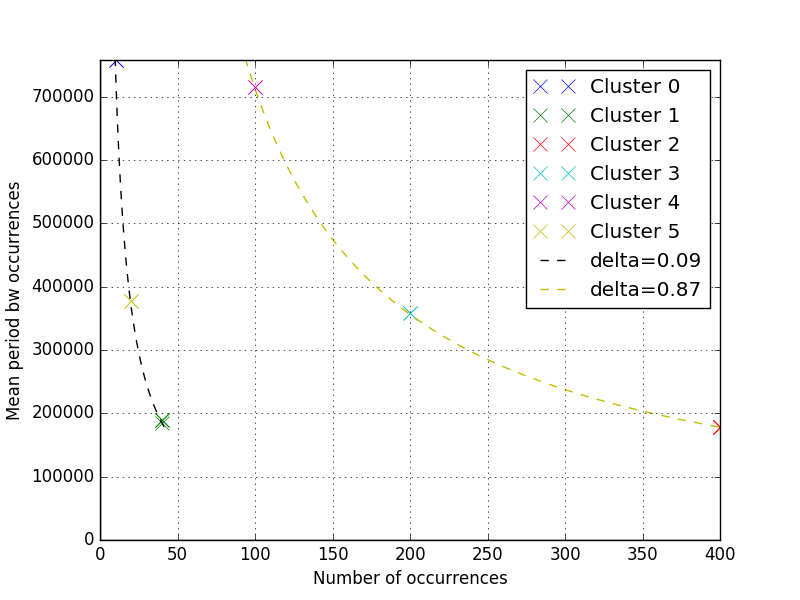
\includegraphics[width=0.5\textwidth]{delta_clustering_test_1}
    \caption{Geometrical representation of delta classification}
    \label{fig:delta_classification_1}
  \end{figure}
  \vfill \null
\end{multicols}

As you can see on figure above, six loops have been detected (this clustering is
related with the previous step not with this last explained delta clustering) 
and classified into two delta groups. The two groups are depicted by these two,
black and yellow curves. So one cluster belongs to one delta if it lies over 
the curve. These curves are described by the function:
$$
f(x)=\frac{\delta*T_{exe}}{x} \text{ being }  0 < \delta \leq 1
$$

Value of $\delta$ is always upper bounder per $1$. It is obvious since one loop
can not have been executed during more time that the entire application time.
Also is lower bounded by zero because if one loop duration is 0 obviously is
would mean it has not been executed. 

Additionally for simplify the loops merging, delta also can be used for
filtering low representative loops. This functionality can be applied even
just after the construction of the $\Omega$ set (reduction step) since at that
point we already have the enough information for calculate $\delta$. Normally,
the lower bound value is set to $0,1$ i.e. It is filtering all loops that
represents less than the 10\% of the overall execution.

On pseudocode \ref{pc:loops_merge_step} there is the actual implementation of
this step. At the very beginning it can be seen how the grouping of the
different loops by deltas is performed, now $\delta$ are subsets of
$\Upsilon$, being $\Delta$ the set of all $\delta$.

\begin{pseudocode}{Loops merge step}{\Upsilon}
\label{pc:loops_merge_step}
    \Delta \GETS deltaClassification(\Upsilon) \\
    \FORALL \delta \in \Delta \DO 
    \BEGIN
        \COMMENT{Sort by it($\upsilon$) desc} \\
        sort(\upsilon \in \delta) \\
        \FOR i \in [0, |\delta|-1) \DO
        \BEGIN
            \FOR j \in [i+1, |\delta|) \DO
            \BEGIN
              \IF isSubloop(\delta_{i}, \delta{j}) \THEN
                  \delta_{i} \mapsto \delta{j} \\
            \END
        \END
    \END
\end{pseudocode}

The key point of this
algorithm is the $isSubloop$ function. Imagine that we have one set of three loops
a, b and c with same $\delta$ with 100, 50 and 10 iterations respectively. 
For sure all three are in a some way related between them but there are two options:
\begin{enumerate*}[label=\roman*)]
    \item $a \mapsto b \mapsto c$
    \item or $a \mapsto c$ and $b \mapsto c$
\end{enumerate*}. You can see the same example where the second option is the
correct on pseudocode
\ref{pc:delta_classification_example_2} and figure
\ref{fig:delta_classification_2}.

\begin{multicols}{2}
  \begin{pseudocode}{Delta example 2}{ }
  \label{pc:delta_classification_example_2}
      \FOR 1 \text{ to } 10 \DO 
      \BEGIN 
        \FOR 1 \text{ to } 5 \DO
        \BEGIN 
            someComms() \\
        \END \\
        \FOR 1 \text{ to } 10 \DO
        \BEGIN 
            someComms()\\
        \END \\
        \text{MPI\_Call} \\
      \END \\
  \end{pseudocode}
  \columnbreak
  \begin{figure}[H]
    \centering
    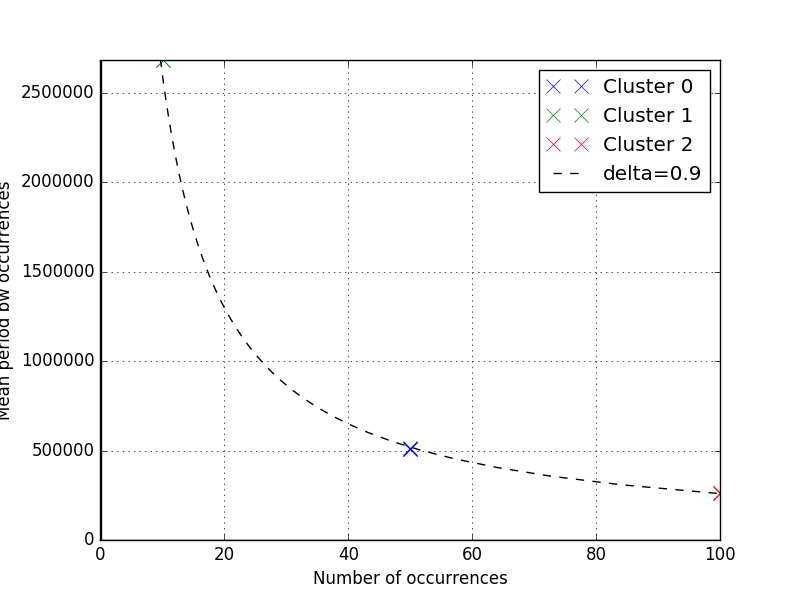
\includegraphics[width=0.5\textwidth]{delta_clustering_test_2}
    \caption{Clustering of delta example 2}
    \label{fig:delta_classification_2}
  \end{figure}
\end{multicols}

In pseudocode \ref{pc:issubloop_function} it can be seen the $isSubloop$ implemented
algorithm. What it does is considering the first mpi call of the target loop
($b$) as the boundaries of its iterations and same think for evaluated loop
($a$). Then the procedure is quite simple, it basically consists in counting how
many iterations of $a$ lies in one iteration of $b$. If any, then $a
\mapsto b$. In the worst case, when $a$ is not subloop of $b$ the
complexity is linear with number of iterations of $b$. Note that the
implications defined in \ref{eq:subloop_rel_imp} are already fulfilled because
the \ref{pc:loops_merge_step} algorithm. Number of iterations of $a$ is greater
than $b$
because the sorting of loops and iteration mean time is lower because both
belongs to the same $\delta$, it means that $it(a)*imt(a) = it(b)*imt(b)$ so $it(a)
> it(b) \Rightarrow imt(a) < imt(b)$

\begin{pseudocode}{IsSubloop function}{a,b}
\label{pc:issubloop_function}
    itBounds \GETS T(firstCall(b)) \\
    subIts \GETS T(firstCall(a)) \\

    \IF subIts_{0} < itBounds_{0} \THEN
        itBounds \GETS \{0\} \cup itBouds \\

    \FOR i \in [0, |itBounds|-1) \DO
    \BEGIN
        lowBound \GETS itBounds_{i} \\
        upBound \GETS itBounds_{i+1} \\

        inIts \GETS \forall x \in inIts : lowBound < x < upBound \\
        \IF |inIts| > 0 \THEN
            \RETURN{True}
    \END \\
    \RETURN{False}
\end{pseudocode}

At the end of this step we already have defined all relations between the
different loops so the actual structure of the application have emerged. 
Internally every time a hierarchical relationship between two loops is found
what the algorithm does is to move the loop from the $\delta$ set to literally
inside the superloop, so at the end of the process on every $\delta \in \Delta$
what we have are the top level loops, defined by:
\begin{equation}
    \label{eq:top_level_loops_de}
    \forall a \in \delta, \nexists b \in \delta: a \mapsto b
\end{equation}

Next step is about representing this information in such a way is easily
understandable to the analyst.

\subsection{Inter-rank reduction}

Until now mpi calls with same call path have been considered different if they 
have been executed by different processes, in this step same call paths from 
different processes are merged, allowing to rank conditional execution to
emerge. The first step is to perform the inter-rank reduction, and once done,
the consecutive calls and loops with same processes are grouped into conditional
blocks, easing the later step of pseudo-code construction.

In pseudocode \ref{pc:inter_rank_reduction} there is a description of how the
inter-rank reduction is done. This function is called for every top level loops
derived from the previous step. Assuming all items in the loop pased as
parameter are ordered by call path, since same call path calls will be
consecutive, the process of reducing is just about traverse the sequence of
items and being collapsing same call path calls.

Remember that call paths consists on a sequence of pairs $(line, file)$. The
only way to order them is by the value of line, so what we do when comparing two
call paths is going from the top stack level to the bottom until there is 
a difference. Since it can be assumed two different branches are done from two 
different lines, the stack level after the last common level will be on same 
file, so here is where the sort takes place taking the line value.

\begin{pseudocode}{Inter rank reduction}{topLevelLoop}
\label{pc:inter_rank_reduction}
    \COMMENT{Get set of mpi calls and subloops} \\
    items \GETS items(topLevelLoop) \\
    \FOR i \in [0, |topLevelLoop|) \DO
    \BEGIN
      \IF isLoop(items_{i}) \THEN
        InterRankReduction(items_{i}) \\
      \ELSE
      \BEGIN
        \FOR j \in [i+1, |topLevelLoop|) \DO
        \BEGIN
          \IF isLoop(items_{j}) \THEN
          \BEGIN
            InterRankReduction(items_{j}) \\
            break \\
          \END
          \ELSE
          \BEGIN
            \IF sameCallPath(item_{i}, item_{j}) \THEN
            \BEGIN
                reduce(item_{i}, item_{j}) \\
                toremove(item_{j}) \\
            \END
            \ELSE
                break \\
          \END
        \END
      \END
    \END
\end{pseudocode}

The last step about group calls/loops into conditional blocks is a similar
construction as before. It just travers all calls and group all consecutive
calls/paths that are executed by the same set of processes. Every time a new
call/loop presents to be executed by a different set of processes a new
conditional block is built up.

\subsection{Pseudo-code construction}

The last step is about representation of the analysis. It is the interface with
the user so is mandatory to provide a way to be as clear as possible. The
information that we want to show is not just an static representation where the
position in code is quite clear but not the order on time, neither just a
temporal representation of the events but a mix of both. We want to show a
temporal representation of events, so its dynamic aspect with clear information
about its possition on code. Additionally we want to attach performance
information for the transitions between mpi calls that are indeed the actual
computation. The alternative that we have found have been represent the
application structure by means of a pseudocode. A toy example is depicted 
in figure \ref{fig:console_gui_example_1}.

\begin{figure}[]
  \centering
  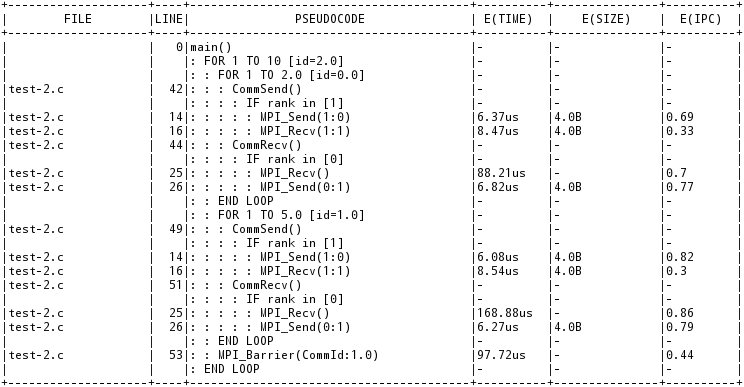
\includegraphics[width=\textwidth]{console_gui_example_1}
  \caption{Console GUI example}
  \label{fig:console_gui_example_1}
\end{figure}

In this example it can be seen that the output consists on 7 columns: 
\begin{description}
  \item \texttt{FILE} Indicates the file from the call of the same line have
    been taken place.
  \item \texttt{LINE} Indicates the precise position in \texttt{FILE} where the
    call in same line have been taken place.
  \item \texttt{PSEUDOCODE} The actual representation of the structure of the
    application. Here you can see the loops and conditional structures when
    there is a divergence among ranks executions. Additionally it can be seen
    the call path taken for every mpi call. About mpi calls there is information
    about partner ranks in the parenthesis.
  \item \texttt{E(time)} Is the mean time in every mpi call.
  \item \texttt{E(size)} Is the mean size of the messages sended/recieved for
    every mpi call
  \item \texttt{E(IPC)} Mean IPC both inside and outside mpi calls. In case of
    figure \ref{fig:console_gui_example_1} there is not information about cpu
    burst in between mpis, in next examples it will be shown.
\end{description}

Additionally an interactive shell have been developed, it allows you to perform
actions like show the cpu burst metrics, filter them by a given thresshold,
filter information by mpi rank, show up the clustering plot and even communicate
with Paraver for show up a trace segment that corresponds to a given iteration
of a given loop. 

The process of transform the internal representation of the structure to the
pseudocode is quite direct. First steps is about remove repetitive information
by means of functions \texttt{extractCommonCallstacks} and
\texttt{hideContiguousCallstacks}. The former is about remove the common
callstack shared by all calls/subloops belonging to the same conditional block
or loop. Even if it can remove most of the repetitive information, there are
cases where there is still information that is repeated but not common to the
whole block, for this cases the second function is the responsible to remove it.
It is better to understand with an example. In pseudocode \ref{pc:beautify_1} is
the original output with all call path information for all mpi call. After
extract the common callstack, we have the scenario depicted in
\ref{pc:beautify_2} where there still are repeated information. Finally after
remove contiguous call path we have \ref{pc:beautify_3}.

\begin{multicols}{3}
\begin{pseudocode}{Orig.}{ }
  \label{pc:beautify_1}
  \FOR 1 \text{ to } N \DO
  \BEGIN
    a:1 \rightarrow b:1 \rightarrow mpi \\
    a:1 \rightarrow b:1 \rightarrow mpi \\
    a:1 \rightarrow b:2 \rightarrow mpi \\
    a:1 \rightarrow b:2 \rightarrow mpi \\
  \END
\end{pseudocode}
\columnbreak
\begin{pseudocode}{Step 1}{ }
  \label{pc:beautify_2}
  a:1 \rightarrow \\
  \FOR 1 \text{ to } N \DO
  \BEGIN
    b:1 \rightarrow mpi \\  
    b:1 \rightarrow mpi \\
    b:2 \rightarrow mpi \\
    b:2 \rightarrow mpi \\
  \END
\end{pseudocode}
\columnbreak
\begin{pseudocode}{Step 2}{ }
  \label{pc:beautify_3}
  a:1 \rightarrow \\
  \FOR 1 \text{ to } N \DO
  \BEGIN
    b:1 \\
     \rightarrow mpi \\
     \rightarrow mpi \\
    b:2 \\
     \rightarrow mpi \\
     \rightarrow mpi \\
  \END
\end{pseudocode}
\end{multicols}

After remove repetitive information, next step is the parsing itself. We leave 
from having a set of phases $\Delta$ that
consists on a set of top level loops, these loops consists on a set of mpi calls 
and other inner loops, so the point is to iterate over every delta, then over 
every loop and finally over every mpi call as is depicted in pseudocodes 
\ref{pc:pseudocode_construction} and \ref{pc:parse_loop_func}.

\begin{pseudocode}{Pseudocode construction}{\Delta}
\label{pc:pseudocode_construction}
    \COMMENT{Sort the top level loops by code position.} \\
    \Delta \GETS sort(\Delta) \\
    \FORALL \delta \in \Delta \DO
    \BEGIN
        \FORALL \upsilon \in \delta \DO
        \BEGIN
          extractCommonCallstacks(\upsilon) \\
          hideContiguousCallstacks(\upsilon) \\
        \END
    \END \\
    \\
    \FORALL \delta \in \Delta \DO
    \BEGIN
        \FORALL \upsilon \in \delta \DO
        \BEGIN
            parseLoopr(\upsilon) \\
        \END
    \END
\end{pseudocode}

\begin{pseudocode}{ParseLoopr}{loop}
\label{pc:parse_loop_func}
    \COMMENT{Sort calls and inner loops by code position} \\
    loop \GETS sort(loop) \\

    \FORALL item \in loop \DO
    \BEGIN
        \IF item \in \Upsilon \THEN
            parseLoopr(item)
        \ELSE
            togui(item)
    \END
\end{pseudocode}
